\documentclass[aspectratio=169,11pt]{ctexbeamer}

\usetheme{Madrid}
\usecolortheme{default}
\setbeamertemplate{navigation symbols}{}
\setbeamertemplate{footline}[frame number]

\usepackage{graphicx}

\definecolor{MainBlue}{RGB}{18,72,120}
\definecolor{SoftBlue}{RGB}{239,246,255}

\setbeamercolor{title}{fg=MainBlue}
\setbeamercolor{frametitle}{fg=MainBlue}
\setbeamercolor{block title}{bg=MainBlue!10,fg=MainBlue}
\setbeamercolor{block body}{bg=SoftBlue,fg=black}

\title{论文汇报}
\subtitle{When Does Concept-Level Aggregation Help?}
\author{基于最新版 main final 整理}
\date{\today}

\begin{document}

\begin{frame}
  \titlepage
\end{frame}

\begin{frame}{研究问题}
  \begin{block}{论文关注的核心问题}
    在联邦学习场景下，如果不同数据之间存在明显差别，那么训练时到底应该：
    \begin{itemize}
      \item 把所有数据合在一起训练；
      \item 还是按不同类别分别训练。
    \end{itemize}
  \end{block}

  \vspace{0.5em}
  \begin{block}{论文想回答的不是}
    不是“怎样设计一个更复杂的方法”，而是回答一个更基础的问题：\textbf{什么时候适合合在一起，什么时候适合分开。}
  \end{block}
\end{frame}

\begin{frame}{研究方法}
  \begin{block}{论文的做法}
    \begin{enumerate}
      \item 先建立一个简化但清晰的分析框架；
      \item 在这个框架下比较“合在一起训练”和“分别训练”的优缺点；
      \item 给出一个判断边界；
      \item 再用模拟实验和真实图片数据验证这个判断。
    \end{enumerate}
  \end{block}

  \vspace{0.5em}
  \begin{block}{核心思想}
    如果不同类别之间差别很明显，那么混在一起训练会互相干扰；\\[0.3em]
    如果差别不大，那么合在一起训练通常更稳定。
  \end{block}
\end{frame}

\begin{frame}{理论部分 1：命题与符号}
  \begin{block}{主要符号}
    \small
    $K$：客户端数量 \quad
    $C$：类别/概念数量 \quad
    $n$：每个客户端的样本数 \\[0.4em]
    $d$：特征维度 \quad
    $\sigma^2$：噪声强度 \quad
    $B_j^2$：第 $j$ 类与整体平均之间的差异
  \end{block}

  \vspace{0.4em}
  \begin{block}{命题：两种训练方式的风险分解}
    \small
    \[
    \mathbb{E}[R_{\text{合在一起}}] = B_j^2 + \frac{\sigma^2 d}{Kn}
    \]
    \[
    \mathbb{E}[R_{\text{分别训练}}] = \frac{\sigma^2 d}{(K/C)n}
    \]
  \end{block}
\end{frame}

\begin{frame}{理论部分 2：核心定理}
  \begin{block}{定理：什么时候按类别分别训练更好}
    \small
    定义
    \[
    \mathrm{SNR}_{\mathrm{concept}}=\frac{Kn B_j^2}{\sigma^2 d}
    \]
    则
    \[
    \text{按类别分别训练更好}\iff \mathrm{SNR}_{\mathrm{concept}} > C-1
    \]
  \end{block}

  \vspace{0.4em}
  \begin{block}{定理结论}
    \small
    类别差异越大、总样本越多时，更适合分别训练；\\[0.3em]
    噪声越大、维度越高、类别越多时，更倾向合在一起训练。
  \end{block}
\end{frame}

\begin{frame}{实验结果 1：什么时候该分开训练？}
  \begin{columns}[T]
    \begin{column}{0.60\textwidth}
      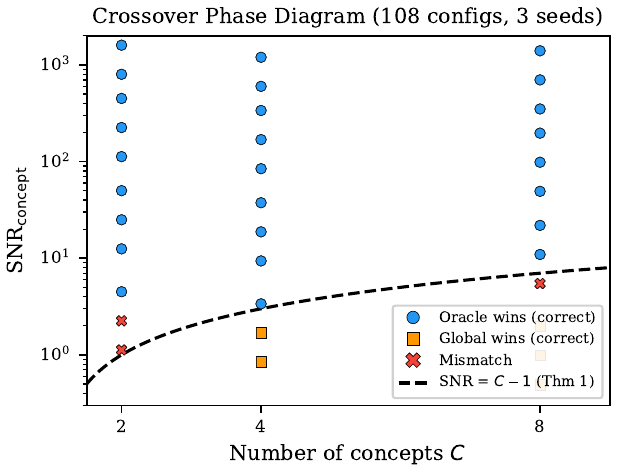
\includegraphics[width=\linewidth]{../figures/phase_diagram.png}
    \end{column}
    \begin{column}{0.38\textwidth}
      \begin{block}{图中结论}
        \begin{itemize}
          \item 左下区域：合在一起训练更稳；
          \item 右上区域：分别训练效果更好；
          \item 大多数实验点都符合这个趋势。
        \end{itemize}
      \end{block}

      \vspace{0.4em}
      \begin{block}{说明}
        这张图说明：\\[0.2em]
        \textbf{分别训练并不是永远更好，而是要看不同数据之间的差别是否足够大。}
      \end{block}
    \end{column}
  \end{columns}
\end{frame}

\begin{frame}{实验结果 2：模拟实验中的整体表现}
  \begin{columns}[T]
    \begin{column}{0.49\textwidth}
      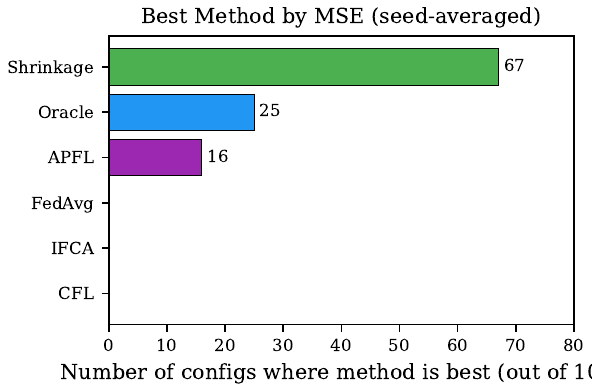
\includegraphics[width=0.96\linewidth]{../figures/best_method.png}
      \vspace{0.2em}
      \begin{block}{左图说明}
        在 108 组设置中，能够根据情况自动调整的做法表现最好。
      \end{block}
    \end{column}
    \begin{column}{0.49\textwidth}
      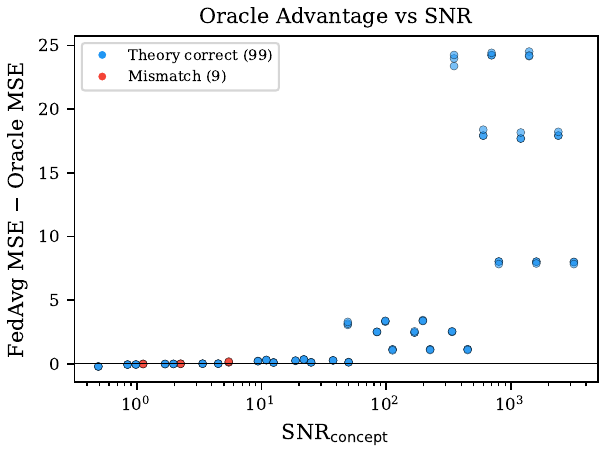
\includegraphics[width=0.96\linewidth]{../figures/snr_advantage.png}
      \vspace{0.2em}
      \begin{block}{右图说明}
        不同类别之间差别越大，分别训练带来的收益就越明显。
      \end{block}
    \end{column}
  \end{columns}
\end{frame}

\begin{frame}{实验结果 3：变化刚发生时的表现}
  \begin{columns}[T]
    \begin{column}{0.58\textwidth}
      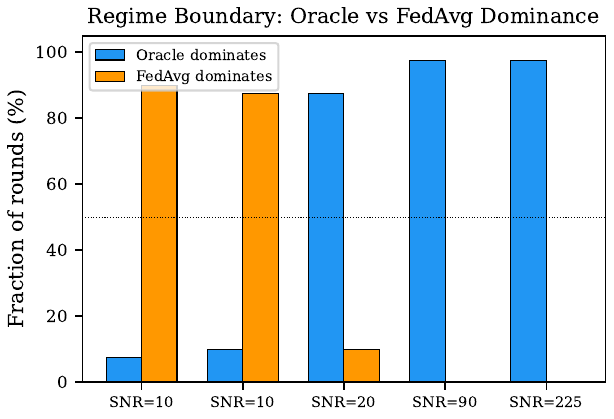
\includegraphics[width=0.96\linewidth]{../figures/regime_boundary.png}
    \end{column}
    \begin{column}{0.40\textwidth}
      \begin{block}{图中现象}
        \begin{itemize}
          \item 从长期看，分别训练可能更好；
          \item 但在变化刚发生时，信息还不够；
          \item 这时先合在一起训练往往更稳。
        \end{itemize}
      \end{block}

      \vspace{0.4em}
      \begin{block}{说明}
        论文不仅回答“要不要分开”，也说明了\textbf{在不同阶段，选择可能不同。}
      \end{block}
    \end{column}
  \end{columns}
\end{frame}

\begin{frame}{实验结果 4：真实图片数据上的结果}
  \begin{columns}[T]
    \begin{column}{0.62\textwidth}
      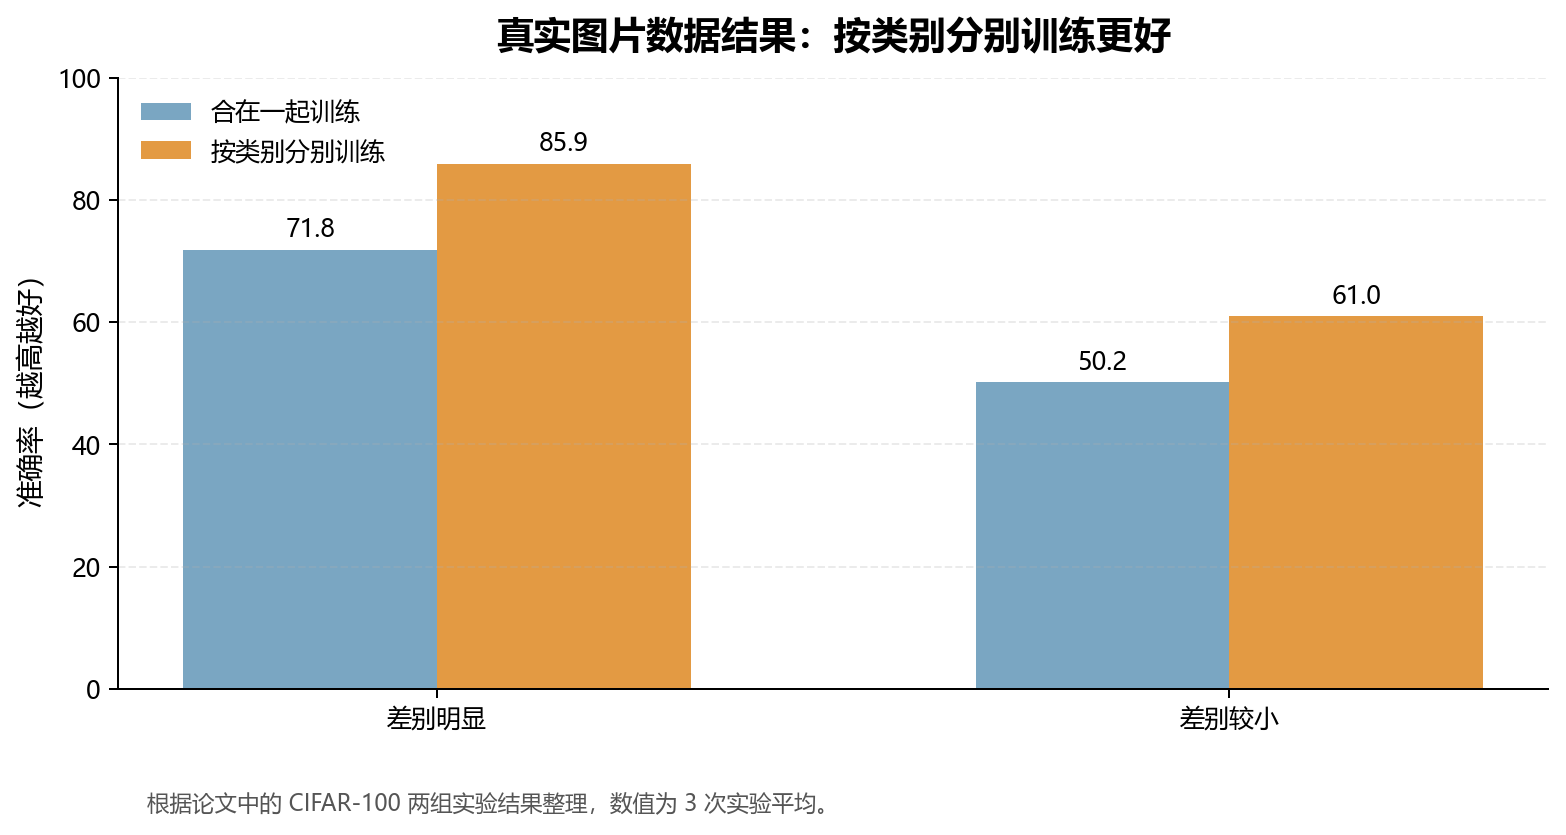
\includegraphics[width=\linewidth]{assets/cifar_bridge_cn.png}
    \end{column}
    \begin{column}{0.36\textwidth}
      \begin{block}{主要结果}
        \begin{itemize}
          \item 我把论文中的真实数据结果整理成了柱状图；
          \item 无论差别明显还是差别较小；
          \item 按类别分别训练都优于合在一起训练。
        \end{itemize}
      \end{block}

      \vspace{0.4em}
      \begin{block}{说明}
        这表明论文中的结论不仅出现在模拟实验里，在真实图片数据上也能观察到。
      \end{block}
    \end{column}
  \end{columns}
\end{frame}

\begin{frame}{结论}
  \begin{block}{论文的主要结论}
    \textbf{并不是所有情况下都应该分别训练。}\\[0.5em]
    当不同类别之间差别明显时，分别训练更好；\\[0.3em]
    当差别不大时，合在一起训练通常更稳。
  \end{block}

  \vspace{0.6em}
  \begin{block}{论文的主要贡献}
    这篇论文把一个过去主要依赖经验判断的问题，变成了一个可以分析、可以验证、也可以指导实际选择的问题。
  \end{block}
\end{frame}

\end{document}
